The most intricate part of the derivation process is processing comprehensions
and aggregates. For both of them, we need to perform as many derivations as the
database allows, therefore we need to deterministically check the contents of
the database until no more derivations are possible.  The matching process is
then similar to the process used for matching a rule's LHS as presented in
Section~\ref{sec:lld_body_match}, however we use two continuation stacks,
$\lstack{C}$ and $\lstack{P}$. In $\lstack{P}$, we put all the initial
persistent frames and in $\lstack{C}$ we put the first linear frame and then
everything else.

In order to reuse the stacks $\lstack{C}$ and $\lstack{P}$, we need to update
them by removing all the frames in $\lstack{C}$ pushed after the first linear
continuation frame.  If we tried to use those frames, we would assumed that the
linear facts used by the other frames were still in the database, but that is
not true because they have been consumed during the first application of the
comprehension.  For example, if the LHS is $\bang \mathtt{a(X)} \otimes
\mathtt{b(X)} \otimes \mathtt{c(X)}$ and the continuation stack has three frames
(one per fact), we cannot backtrack to the frame of $\mathtt{c(X)}$ because, at
that point, the matching process was assuming that the previous \texttt{b(X)}
linear fact was still available.  Moreover, we also need to remove the consumed
linear facts from the frames of \texttt{b(X)} and $\bang$\texttt{a(X)} in order
to make the stack fully consistent with the new database. We will see later on
how to do that.

\subsubsection{Example}

As an example, consider the following snippet of code inspired in the PageRank
program shown in Fig.~\ref{language:code:async_pagerank}:

\begin{Code}
update(A),
!numInbound(A, T)
   -o [sum => V; B, W, Val | !edge(A, B), neighbor-pagerank(A, B, Val),
         V = Val/float(T) -o neighbor-pagerank(A, B, Val) -> sum-ranks(A, V)].
\end{Code}

Let's assume that the rule above was successfully matched with \code{A = 1} and
\code{T = 2} and the database contains the following facts: \code{\bang edge(1,
2)}, \code{\bang edge(1, 3)}, \code{neighbor-pagerank(1, 2, 0.5)} and
\code{neighbor-pagerank(1, 3, 0.5)}. Figure~\ref{fig:logic:backtrack} shows how
the aggregate is computed using the continuation stack. An initial frame is
created for \code{\bang edge(1, B)} which includes two \code{edge} facts and
\code{\bang edge(1, 2)} is selected to continue the process. Since \code{B = 2},
the frame for \code{neighbor-pagerank(1, 2, Val)} includes only
\code{neighbor-pagerank(1, 2, 0.5)} which completes the first application of the
aggregate and the same linear fact is re-derived using the first aggregate's
RHS.  Computation then proceeds by backtracking to the first linear frame, the
frame of \code{neighbor-pagerank(1, 2, Val)}, but there are no more available
candidates, therefore the frame is removed and the next candidate \code{\bang
edge(1, 3)} of frame \code{\bang edge(1, B)} is selected. Here, a frame is
created for \code{B = 3} with \code{neighbor-pagerank(1, 3, 0.5)} and the second
application of the aggregate is completed. The process backtracks again twice
but now there are no more candidates and the second aggregate's RHS derives
\code{sum-ranks(1, 1.0)} because \code{V = 0.5 + 0.5}, completing the aggregate
computation.

\begin{figure}[ht]
   \begin{center}
      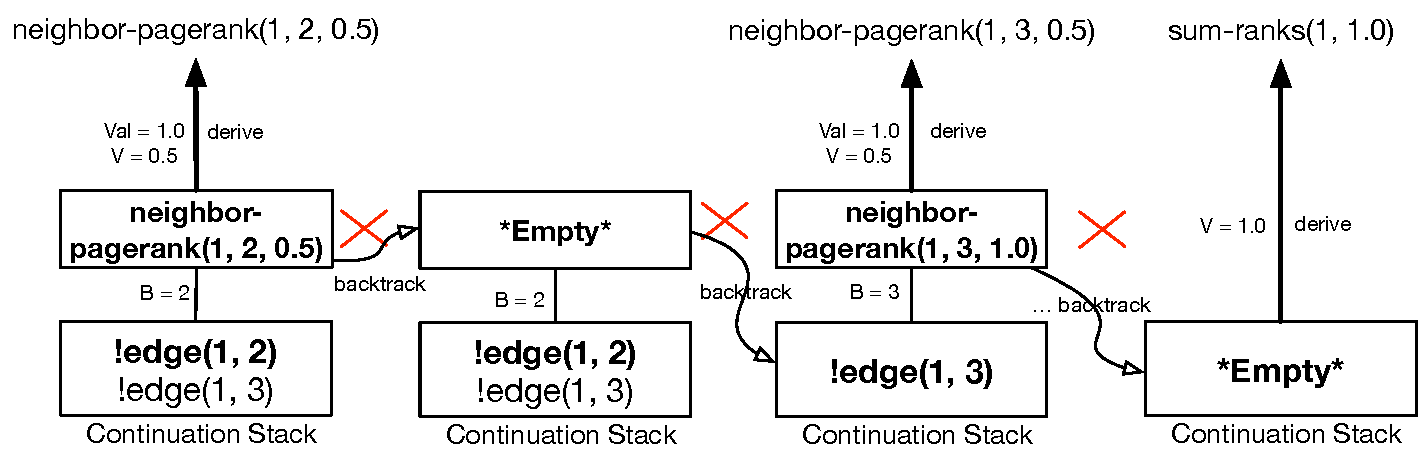
\includegraphics[width=0.85\linewidth]{figures/logical_foundations/backtrack.pdf}
   \end{center}
   \mycap{Generating the PageRank aggregate.}
   \label{fig:logic:backtrack}
\end{figure}

\subsubsection{Matching}

The matching state for aggregates is 
$\matstatea{\deltan}{\lstack{C};
   \lstack{P}}{\Gamma}{\Delta}{\Omega}{\Delta' \rightarrow \Omega'}{\Sigma}$

\begin{enumerate}

   \item[$\omegan$] ordered list of remaining terms of the rule's RHS to be
      derived;

   \item[$\deltan$] multi-set of linear facts that were still available after
      matching the rule's LHS and all the previous aggregates. Note that
      $\Delta, \Xi = \deltan$;

   \item[$\Xi$] multi-set of linear facts used during the matching process of
      the rule's LHS and all the previous aggregates;

   \item[$\Gamma_{1}$] set of persistent facts derived up to this point in the
   rule's RHS;

   \item[$\Delta_{1}$] multi-set of linear facts derived up to this point in
   the rule's RHS;

   \item[$\Delta'$] multi-set of linear facts consumed up to this point;

   \item[$\Omega'$] terms matched using $\Delta'$ up to this point;

   \item[$\m{agg}$] aggregate that is being matched;

   \item[$\Sigma$] the list of aggregated values;

   \item[$\lstack{C}$] continuation stack that contains both linear and persistent
   frames. The first frame must be linear;

   \item[$\lstack{P}$] initial part of the continuation stack with only persistent
   frames;

   \item[$\Delta$] multi-set of linear facts remaining up to this point in the
   matching process;

   \item[$\Omega$] ordered list of terms that need to be matched for the
   comprehension to be applied.

\end{enumerate}

Since aggregates accumulate values (from specific variables), we retrieved the
value from the $\Psi$ context. Remember that $\Psi$ is used for the
quantification connectives in the sequent calculus and in LLD is used to store
current variable bindings.

\subsubsection{Linear atomic propositions}

The following two transitions deal with the case when there is a linear
atomic propositions in the aggregates' LHS.


\begin{multline}
\transx{
   \matstatea{\deltan}{\lstack{C};
      \lstack{P}}{\Gamma}{\Delta, p_1, \Delta''}{p, \Omega}{\Delta' \rightarrow
         \Omega'}{\Sigma}
}
{
   \matstatea{\deltan}{\lframe{\Delta,
   p_1}{\Delta''}{p}{\Omega}{\Delta'}{\Omega'}, \lstack{C}; \lstack{P}}{\Gamma}{\Delta,
      \Delta''}{\Omega}{\Delta', p \rightarrow \Omega' \otimes
      p}{\Sigma}\tag{agg match p ok}
}
\end{multline}

\[
\trans{
   \matstatea{\deltan}{\lstack{C}; \lstack{P}}{\Gamma}{\Delta}{p,
      \Omega}{\Delta' \rightarrow \Omega'}{\Sigma}
}
{
   \contstatea{\deltan}{\lstack{C} ; \lstack{P}}{\Gamma}{\Sigma}
}\tag{agg match p fail}
\]


\subsubsection{Persistent atomic propositions}

The transitions for dealing with persistent facts are similar to the previous
ones.



\[
\trans{
   \matstatea{\Delta_N}{\cdot;
      \lstack{P}}{\Gamma, p_1, \Gamma''}{\Delta}{\bang p, \Omega}{\Delta' \rightarrow
         \Omega'}{\Sigma}
}
{
   \matstatea{\Delta_N}{\cdot; \pframe{\Gamma''}{\Delta}{\bang
   p}{\Omega}{\Delta'}{\Omega'}, \lstack{P}}{\Gamma, p_1, \Gamma''}{\Delta}{\Omega}
   {\Delta' \rightarrow \Omega' \otimes \bang p}{\Sigma}
}
\]

\[
\trans{
   \matstatea{\Delta_N}{\lstack{C};
      \lstack{P}}{\Gamma, p_1, \Gamma''}{\Delta}{\bang p, \Omega}{\Delta' \rightarrow
         \Omega'}{\Sigma}
}
{
   \matstatea{\Delta_N}{\pframe{\Gamma''}{\Delta}{\bang
   p}{\Omega}{\Delta'}{\Omega'}, \lstack{C} ; \lstack{P}}{\Gamma, p_1, \Gamma''}{\Delta}{\Omega}
   {\Delta' \rightarrow \Omega' \otimes \bang p}{\Sigma}
}
\]


\[
\trans{
   \matstatea{\Delta_N}{\lstack{C}; \lstack{P}}{\Gamma}{\Delta}{\bang p,
      \Omega}{\Delta' \rightarrow \Omega'}{\Sigma}
}
{
   \contstatea{\Delta_N}{\lstack{C} ; \lstack{P}}{\Gamma}{\Sigma}
}
\]



\subsubsection{LHS Deconstruction}


\begin{multline}
\transx{
   \matstatea{\deltan}{\lstack{C};
      \lstack{P}}{\Gamma}{\Delta}{X \otimes Y, \Omega}{\Delta' \rightarrow
         \Omega'}{\Sigma}
}
{
   \matstatea{\deltan}{\lstack{C};
      \lstack{P}}{\Gamma}{\Delta}{X, Y, \Omega}{\Delta' \rightarrow
         \Omega'}{\Sigma}
} \tag{agg match $\otimes$}
\end{multline}

\begin{multline}
\transx{
   \matstatea{\deltan}{\lstack{C};
      \lstack{P}}{\Gamma}{\Delta}{\one, \Omega}{\Delta' \rightarrow
         \Omega'}{\Sigma}
}
{
   \matstatea{\deltan}{\lstack{C};
      \lstack{P}}{\Gamma}{\Delta}{\Omega}{\Delta' \rightarrow
         \Omega'}{\Sigma}
      } \tag{agg match $\one$}
\end{multline}



\subsubsection{Successful match}

When the aggregate's LHS finally matches, we retrieve the term for variable $x$
(the aggregate variable) and add it to the list $\Sigma$.

\[
\infer[\ma{AG} \m{end}]
{\ma{AG} \Psi; \Gamma; \Delta; \Xi_N; \Gamma_{N1}; \Delta_{N1}; \Xi; \cdot;
   \lstack{C}; \lstack{P}; \Omega_N; \Delta_N; \Sigma \rightarrow \outsem}
{\fixa{AG} \Gamma; \Xi_N; \Gamma_{N1}; \Delta_{N1}; \Xi; \lstack{C}; \lstack{P}; \Omega_N;
   \Delta_N; V :: \Sigma \rightarrow \outsem & x : V : \tau \in \Psi}
\]


\subsubsection{Continuation stack update}

As we said before, to update the continuation stacks, we need remove to all the
frames except the first linear frame and remove the consumed linear facts from
the remaining frames so that they are still valid for the next application of
the aggregate.  The judgment that updates the stack has the form
$\fixstatea{\Delta}{\Xi; \Delta'}{\lstack{C};
   \lstack{P}}{\Gamma}{\Sigma}$, where:

\begin{enumerate}

   \item[$\omegan$] ordered list of remaining terms of the rule's RHS to be
      derived;

   \item[$\Delta$] multi-set of linear facts that were still available after
   matching the rule's LHS and the aggregate's LHS;
   \item[$\Xi$] multi-set of linear facts used during the matching process of
   the rule's LHS and all the previous aggregates;
   \item[$\Delta'$] multi-set of linear facts consumed by the aggregate's LHS;

   \item[$\gammanew$] set of persistent facts derived by the rule's RHS and all
      the previous aggregates;

   \item[$\deltanew$] multi-set of linear facts derived by the rule's RHS and
      all the previous aggregates;

   \item[$\m{agg}$] the current aggregate;
   \item[$\Sigma$] list of accumulated values;
   \item[$\lstack{C}, \lstack{P}$] continuation stacks for the comprehension;
   \item[$\Gamma$] set of usable persistent facts.
\end{enumerate}

\subsubsection{Remove linear continuation frames}

To remove all linear continuation frames except the first one, we simply go
through all the frames in the stack $\lstack{C}$ until only one frame remains.
This last frame and stack $\lstack{P}$ are then updated by removing $\Delta'$
from its contexts.


{\tiny
\[
\infer[\fixa ~\m{end~linear}]
{\fixa \Gamma; \Xi_N; \Gamma_{N1}; \Delta_{N1}; \Xi; (\Delta_x; \Delta''; \cdot;
      p; \Omega; \cdot; \Upsilon); P;  \aggsz{A}{B}{C}; \Omega_N; \Delta_N; T \rightarrow \Xi'; \Delta'; \Gamma'}
{\begin{split}\strans &\Xi; P; P' \\ \da \Gamma; \Xi_N, \Xi; \Gamma_{N1};
   \Delta_{N1}; B; (\Delta_x - \Xi; \Delta'' - \Xi; \cdot;& p; \Omega; \cdot;
         \Upsilon) ; P' ; \aggsz{A}{B}{C}; \Omega_N; (\Delta_N - \Xi); T &\rightarrow \Xi'; \Delta'; \Gamma'\end{split}}
\]
}

\[
\infer[\fixa \m{more}]
{\fixa \Gamma; \Xi_N; \Gamma_{N1}; \Delta_{N1}; \Xi; \_, X, C; P; AG; \Omega_N; \Delta_N; T \rightarrow \Xi'; \Delta'; \Gamma'}
{\fixa \Gamma; \Xi_N; \Gamma_{N1}; \Delta_{N1}; \Xi; X, C; P; AG; \Omega_N; \Delta_N; T \rightarrow \Xi'; \Delta'; \Gamma'}
\]

{\footnotesize
\[
\infer[\fixa \m{end~empty}]
{\fixa \Gamma; \Xi_N; \Gamma_{N1}; \Delta_{N1}; \Xi; \cdot; P; \aggsz{A}{B}{C}; \Omega_N; \Delta_N; T \rightarrow \Xi'; \Delta'; \Gamma'}
{\begin{split}\strans &\Xi; P; P' \\ \da \Gamma; \Xi_N, \Xi; \Gamma_{N1};
   \Delta_{N1}; B; \cdot ; P' ; &\aggsz{A}{B}{C}; \Omega_N; (\Delta_N - \Xi); T &\rightarrow \Xi'; \Delta'; \Gamma'\end{split}}
\]
}


\subsubsection{Aggregate backtracking}

If the aggregate match fails, we need to backtrack to the next candidate fact.
The backtracking state 
has the form
$\contstatea{\deltan}{\lstack{C} ; \lstack{P}}{\Gamma}{\Sigma}$, where:

\begin{enumerate}

   \item[$\omegan$] ordered list of remaining terms of the rule's RHS to be
      derived;

   \item[$\deltan$] multi-set of linear facts that were still available after
   matching the rule's LHS and the aggregate's LHS;
   \item[$\Xi$] multi-set of linear facts used during the matching process of
   the rule's LHS and all the previous aggregates;

   \item[$\gammanew$] set of persistent facts derived by the rule's RHS and all
      the previous aggregates;

   \item[$\deltanew$] multi-set of linear facts derived by the rule's RHS and
      all the previous aggregates;

   \item[$\m{agg}$] the current aggregate;
   \item[$\Sigma$] list of accumulated values.
   \item[$\lstack{C}, \lstack{P}$] continuation stacks for the comprehension;
   \item[$\Gamma$] set of usable persistent facts.
\end{enumerate}

\paragraph{Using the $\lstack{C}$ stack}

The following 4 state transitions use the $\lstack{C}$ stack, the stack where the
first continuation frame is linear, to perform backtracking.


\begin{multline}
\transx{
   \contstatea{\deltan}{\lframe{\Delta}{p_1, \Delta''}{p}{\Omega}{\Delta'}{\Omega'}, \lstack{C} ; \lstack{P}}{\Gamma}{\Sigma}
}
{
   \matstatea{\deltan}{\lframe{\Delta,
      p_1}{\Delta''}{p}{\Omega}{\Delta'}{\Omega'}, \lstack{C}; \lstack{P}}{\Gamma}{\Delta}{p,
      \Omega}{\Delta', p_1 \rightarrow \Omega' \otimes p}{\Sigma}
} \tag{agg next p $\lstack{C}$}
\end{multline}

\begin{multline}
\transx{
   \contstatea{\deltan}{\pframe{p_1, \Gamma''}{\Delta}{\bang
   p}{\Omega}{\Delta'}{\Omega'}, \lstack{C} ; \lstack{P}}{\Gamma}{\Sigma}
}
{
   \matstatea{\deltan}{\pframe{\Gamma''}{\Delta}{\bang p}
      {\Omega}{\Delta'}{\Omega'}, \lstack{C}; \lstack{P}}{\Gamma}{\Delta}{p,
      \Omega}{\Delta' \rightarrow \Omega' \otimes \bang p}{\Sigma}
} \tag{agg next \bang p $\lstack{C}$}
\end{multline}

\[
\trans{
   \contstatea{\deltan}{\lframe{\Delta}{\cdot}{p}{\Omega}{\Delta'}{\Omega'}, \lstack{C} ; \lstack{P}}{\Gamma}{\Sigma}
}
{
   \contstatea{\deltan}{\lstack{C} ; \lstack{P}}{\Gamma}{\Sigma}
} \tag{agg  next frame $\lstack{C}$}
\]

\[
\trans{
   \contstatea{\deltan}{\pframe{\cdot}{\Delta}{\bang
   p}{\Omega}{\Delta'}{\Omega'}, \lstack{C} ; \lstack{P}}{\Gamma}{\Sigma}
}
{
   \contstatea{\deltan}{\lstack{C} ; \lstack{P}}{\Gamma}{\Sigma}
} \tag{agg next \bang frame $\lstack{C}$}
\]


\paragraph{Using the $\lstack{P}$ stack}

The following 2 state transitions rules use the $\lstack{P}$ stack instead, the stack where all
continuation frames are persistent.

\[
\infer[\conta{AG} \m{next}~\lstack{P}~\bang p]
{\conta{AG} \Gamma; \Delta_N; \Xi_N; \Gamma_{N1}; \Delta_{N1}; \cdot; f, \lstack{P}; \Omega_N; \Sigma \rightarrow \outsem}
{\begin{gathered}
   f = [p_1, \Gamma'; \Delta_N; \cdot; \bang p; \Omega; \cdot; \Upsilon] \\
   f' = [\Gamma'; \Delta_N; \cdot; \bang p; \Omega; \cdot; \Upsilon] \\
   \ma{AG} \Gamma; \Delta_N; \Xi_N; \Gamma_{N1}; \Delta_{N1}; \cdot; \Omega; \cdot;
      f', \lstack{P}; \Omega_N; \Delta_N; \Sigma \rightarrow \outsem
 \end{gathered}
}
\]

\[
\infer[\conta{AG} \m{next}~\lstack{P}~\m{empty}~\bang p]
{\conta{AG} \Gamma; \Delta_N; \Xi_N; \Gamma_{N1}; \Delta_{N1}; \cdot; f, \lstack{P}; \Omega_N; \Sigma
   \rightarrow \outsem}
{\begin{gathered}
   f =  [\cdot; \Delta_N; \cdot; \bang p; \Omega; \cdot; \Upsilon] \\
   \conta{AG} \Gamma; \Delta_N; \Xi_N; \Gamma_{N1}; \Delta_{N1}; \cdot; \lstack{P};
      \Omega_N; \Sigma \rightarrow \outsem
 \end{gathered}
}
\]


\paragraph{Aggregate done}

If both the $\lstack{C}$ and $\lstack{P}$ stacks are empty, backtracking is
impossible and the aggregate is done. The final aggregate's RHS is then derived
along with the rest of the rule's RHS.

\[
\infer[\conta{\aggsz{A}{B}{C}} \m{end}]
{\conta{\aggsz{A}{B}{C}} \Gamma; \Delta_N; \Xi_N; \Gamma_{N1}; \Delta_{N1}; \cdot; \cdot;
   \Omega; \Sigma \rightarrow \outsem}
{\done \Gamma; \Delta_N; \Xi_N; \Gamma_{N1}; \Delta_{N1}; (\lambda x. C
      x)\Sigma,
   \Omega \rightarrow \outsem}
\]


\subsubsection{Aggregate Derivation}

After updating the continuation stacks, the first aggregate's RHS is derived.
The derivation state has the form
$\derstatea{\Delta}{\Xi}{\gammanew}{\deltanew}{\Sigma}{\lstack{C};
\lstack{P}}{\Omega}$, where:

\begin{enumerate}

   \item[$\omegan$] ordered list of remaining terms of the rule's RHS to be
      derived;

   \item[$\Delta$] multi-set of remaining linear facts that can be used for
   the next aggregate applications.

   \item[$\Xi$] multi-set of linear facts consumed both by the rule's LHS and
      previous aggregate applications;

   \item[$\gammanew$] set of persistent facts derived by the rule's RHS, previous
      aggregates and current derivation;

   \item[$\deltanew$] multi-set of linear facts derived by the rule's RHS,
      previous aggregates and current derivation;

   \item[$\m{agg}$] current aggregate symbol;
   \item[$\Sigma$] accumulated list of values of the aggregate;
   \item[$\lstack{C}, \lstack{P}$] new continuation stacks;
   \item[$\Gamma$] set of persistent facts;
   \item[$\Omega$] ordered list of terms to derive.
\end{enumerate}

\[
\infer[\da{AG} p]
{\da{AG} \Gamma; \Delta_N; \Xi_N; \Gamma_1; \Delta_1; p, \Omega; \lstack{C}; \lstack{P}; \Omega_N;
   \Sigma \rightarrow \outsem}
{\da{AG} \Gamma; \Delta_N; \Xi_N; \Gamma_1; \Delta_1, p; \Omega; \lstack{C}; \lstack{P}; \Omega_N;
   \Sigma \rightarrow \outsem}
\]

\[
\infer[\da{AG} \bang p]
{\da{AG} \Gamma; \Delta_N; \Xi_N; \Gamma_1; \Delta_1; \bang p, \Omega; \lstack{C};
   \lstack{P}; \Omega_N; \Sigma \rightarrow \outsem}
{\da{AG} \Gamma; \Delta_N; \Xi_N; \Gamma_1, p; \Delta_1; \Omega; \lstack{C}; \lstack{P}; \Omega_N;
   \Sigma \rightarrow \outsem}
\]

\[
\infer[\da{AG} \otimes]
{\da{AG} \Gamma; \Delta_N; \Xi_N; \Gamma_1; \Delta_1; A \otimes B, \Omega; \lstack{C}; \lstack{P}; \Omega_N;
   \Sigma \rightarrow \outsem}
{\da{AG} \Gamma; \Delta_N; \Xi_N; \Gamma_1; \Delta_1; A, B, \Omega; \lstack{C}; \lstack{P}; \Omega_N;
   \Sigma \rightarrow \outsem}
\]

\[
\infer[\da{AG} \m{end}]
{\da{AG} \Gamma; \Delta_N; \Xi_N; \Gamma_1; \Delta_1; \cdot; \lstack{C}; \lstack{P}; \Omega_N;
   \Sigma \rightarrow \outsem}
{\conta{AG} \Gamma; \Delta_N; \Xi_N; \Gamma_1; \Delta_1; \lstack{C}; \lstack{P}; \Omega_N; \Sigma
   \rightarrow \outsem}
\]



This completes the specification of the LLD semantics.

